\section{Theoretical Background}

The reaction outcome depends strongly on the interaction time scale and on how energy and momentum are shared between nucleons. Three limiting, and often coexisting, mechanisms are particularly relevant: direct reactions, compound-nucleus reactions, and pre-equilibrium emission \cite{preeq_image,koning2025talys}.

\begin{itemize}
\item \textbf{Direct reactions:} In a direct process the projectile interacts with the target through fast steps,
taking the system quickly from the initial to the final state. Direct and direct-like processes tend to
preserve "memory" of the entrance channel\footnote{The entrance channel is the initial projectile--target configuration, including incident energy and direction. `Memory'' means that angular correlations with the incident direction can persist, rather than being largely randomized during equilibration of a long-lived compound nucleus.}
and often produce anisotropic angular distributions\footnote{The emission probability depends on direction:\(d\sigma/d\Omega\) varies with angle, i.e.\ it is not the same for every direction.}.


\item \textbf{Compound-nucleus reactions:} The projectile is absorbed and a highly excited compound nucleus is formed.
If the compound system lives long enough for its excitation energy to be redistributed among many degrees
of freedom, its decay can be treated statistically. This typically yields evaporation-like spectra and
comparatively isotropic emission\footnote{The emission is approximately uniform in angle: \(d\sigma/d\Omega\ \approx \text{constant}\), i.e.\ weak angular dependence.}.

\item \textbf{Pre-equilibrium emission:} Between these two limits lies pre-equilibrium, or pre-compound, emission.
Here particles can be emitted after the first interaction steps but before full statistical equilibration is reached.
Pre-equilibrium emission therefore often contributes substantially to the higher-energy part of the outgoing
spectrum and may remain anisotropic due to partial memory of the entrance channel.

\end{itemize}

The emitted-particle spectrum is usually represented as a function of the outgoing energy, denoted here by \(E_{\mathrm{out}}\). This quantity corresponds to the kinetic energy carried by the emitted particle after the reaction. The different reaction mechanisms are illustrated schematically in \cref{fig:mechanisms_schematic}: compound emission typically produces a Maxwellian-distributed evaporation peak at low \(E_{\mathrm{out}}\), pre-equilibrium emission contributes a harder shoulder extending to higher outgoing energies, and direct-like processes can generate more structured features \cite{preeq_image}.

\begin{figure}[H]
\centering
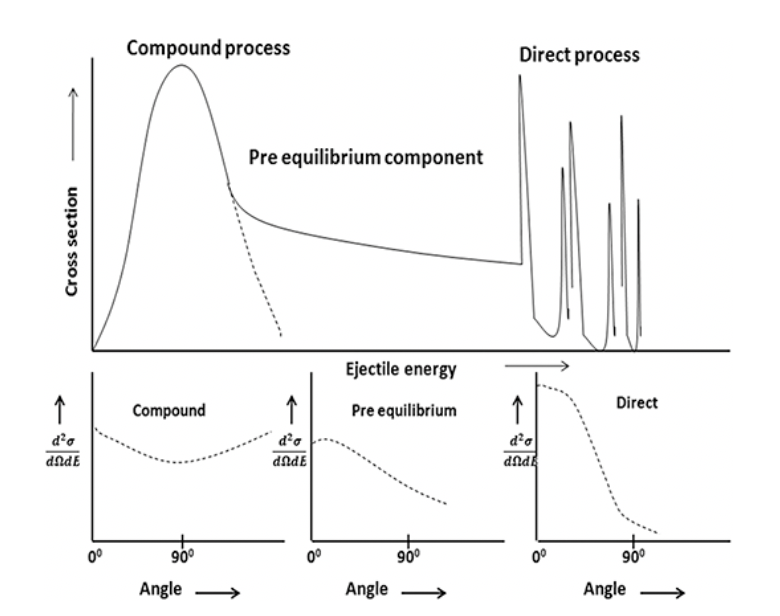
\includegraphics[width=0.45\linewidth]{Images/Energy_Spectrum_Double_cross-section.png}
\caption{Schematic energy spectrum showing typical contributions from compound, pre-equilibrium, and direct-like mechanisms and the typical angular distributions for each component. Adapted from \cite{preeq_image}.}
\label{fig:mechanisms_schematic}
\end{figure}
